\documentclass{standalone}
\usepackage{tikz}
\usetikzlibrary{patterns, positioning}


\begin{document}
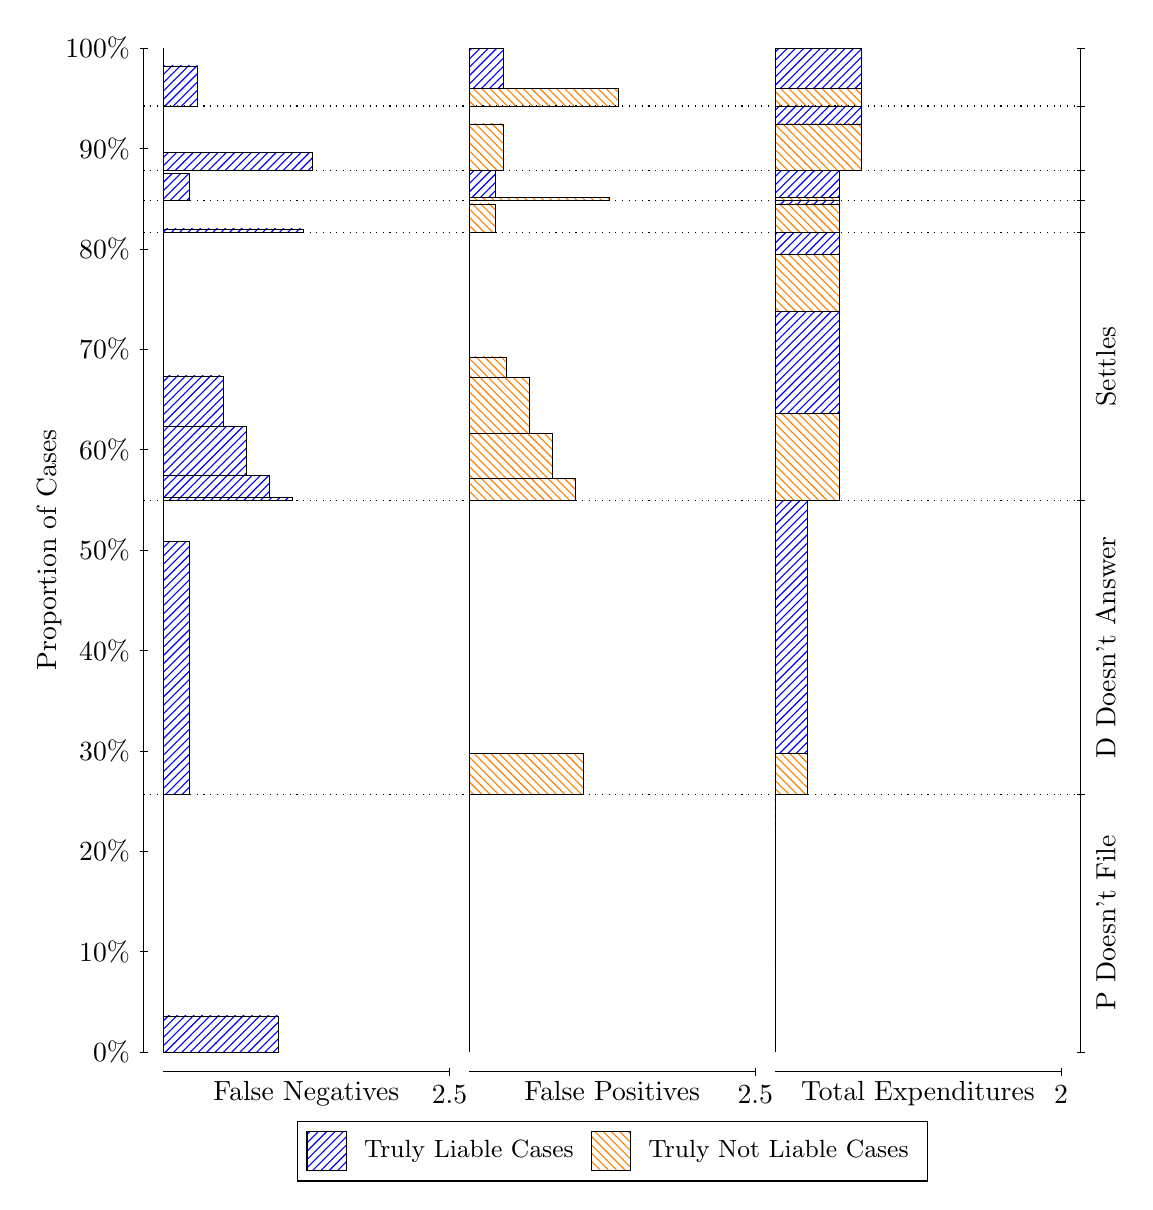
\begin{tikzpicture}
\draw[black, very thin] (1.5,1.75) -- (1.5,14.5);
\node[rotate=90, text=black, anchor=center] at (0.3, 8.125) {Proportion of Cases};
\draw[black, very thin] (1.45,1.75) -- (1.55,1.75);
\node[text=black, anchor=east] at (1.45, 1.75) {0\%};
\draw[black, very thin] (1.45,3.025) -- (1.55,3.025);
\node[text=black, anchor=east] at (1.45, 3.025) {10\%};
\draw[black, very thin] (1.45,4.3) -- (1.55,4.3);
\node[text=black, anchor=east] at (1.45, 4.3) {20\%};
\draw[black, very thin] (1.45,5.575) -- (1.55,5.575);
\node[text=black, anchor=east] at (1.45, 5.575) {30\%};
\draw[black, very thin] (1.45,6.85) -- (1.55,6.85);
\node[text=black, anchor=east] at (1.45, 6.85) {40\%};
\draw[black, very thin] (1.45,8.125) -- (1.55,8.125);
\node[text=black, anchor=east] at (1.45, 8.125) {50\%};
\draw[black, very thin] (1.45,9.4) -- (1.55,9.4);
\node[text=black, anchor=east] at (1.45, 9.4) {60\%};
\draw[black, very thin] (1.45,10.675) -- (1.55,10.675);
\node[text=black, anchor=east] at (1.45, 10.675) {70\%};
\draw[black, very thin] (1.45,11.95) -- (1.55,11.95);
\node[text=black, anchor=east] at (1.45, 11.95) {80\%};
\draw[black, very thin] (1.45,13.225) -- (1.55,13.225);
\node[text=black, anchor=east] at (1.45, 13.225) {90\%};
\draw[black, very thin] (1.45,14.5) -- (1.55,14.5);
\node[text=black, anchor=east] at (1.45, 14.5) {100\%};

\draw[black, very thin] (13.4,1.75) -- (13.4,14.5);
\draw[black, very thin] (13.35,1.75) -- (13.45,1.75);
\node[anchor=west] at (13.35, 1.75) {};
\draw[black, very thin] (13.35,5.025) -- (13.45,5.025);
\node[anchor=west] at (13.35, 5.025) {};
\draw[black, very thin] (13.35,8.7537) -- (13.45,8.7537);
\node[anchor=west] at (13.35, 8.7537) {};
\draw[black, very thin] (13.35,12.159) -- (13.45,12.159);
\node[anchor=west] at (13.35, 12.159) {};
\draw[black, very thin] (13.35,12.564) -- (13.45,12.564);
\node[anchor=west] at (13.35, 12.564) {};
\draw[black, very thin] (13.35,12.947) -- (13.45,12.947);
\node[anchor=west] at (13.35, 12.947) {};
\draw[black, very thin] (13.35,13.764) -- (13.45,13.764);
\node[anchor=west] at (13.35, 13.764) {};
\draw[black, very thin] (13.35,14.5) -- (13.45,14.5);
\node[anchor=west] at (13.35, 14.5) {};

\draw[black, very thin, pattern color=blue, pattern=north east lines] (1.75,1.75) rectangle (3.2033,2.2079);
\draw[black, very thin, pattern color=orange, pattern=north west lines] (1.75,2.2079) rectangle (1.75,5.0251);
\draw[black, very thin, pattern color=blue, pattern=north east lines] (1.75,5.0251) rectangle (2.077,8.2392);
\draw[black, very thin, pattern color=orange, pattern=north west lines] (1.75,8.2392) rectangle (1.75,8.7537);
\draw[black, very thin, pattern color=blue, pattern=north east lines] (1.75,8.7537) rectangle (3.385,8.7891);
\draw[black, very thin, pattern color=blue, pattern=north east lines] (1.75,8.7891) rectangle (3.0943,9.0713);
\draw[black, very thin, pattern color=blue, pattern=north east lines] (1.75,9.0713) rectangle (2.8037,9.6925);
\draw[black, very thin, pattern color=blue, pattern=north east lines] (1.75,9.6925) rectangle (2.513,10.336);
\draw[black, very thin, pattern color=orange, pattern=north west lines] (1.75,10.336) rectangle (1.75,12.159);
\draw[black, very thin, pattern color=blue, pattern=north east lines] (1.75,12.159) rectangle (3.5303,12.202);
\draw[black, very thin, pattern color=orange, pattern=north west lines] (1.75,12.202) rectangle (1.75,12.564);
\draw[black, very thin, pattern color=blue, pattern=north east lines] (1.75,12.564) rectangle (2.077,12.906);
\draw[black, very thin, pattern color=orange, pattern=north west lines] (1.75,12.906) rectangle (1.75,12.947);
\draw[black, very thin, pattern color=blue, pattern=north east lines] (1.75,12.947) rectangle (3.6393,13.174);
\draw[black, very thin, pattern color=orange, pattern=north west lines] (1.75,13.174) rectangle (1.75,13.764);
\draw[black, very thin, pattern color=blue, pattern=north east lines] (1.75,13.764) rectangle (2.186,14.274);
\draw[black, very thin, pattern color=orange, pattern=north west lines] (1.75,14.274) rectangle (1.75,14.5);
\draw[black, very thin, pattern color=orange, pattern=north west lines] (5.6333,1.75) rectangle (5.6333,4.5672);
\draw[black, very thin, pattern color=blue, pattern=north east lines] (5.6333,4.5672) rectangle (5.6333,5.0251);
\draw[black, very thin, pattern color=orange, pattern=north west lines] (5.6333,5.0251) rectangle (7.0867,5.5395);
\draw[black, very thin, pattern color=blue, pattern=north east lines] (5.6333,5.5395) rectangle (5.6333,8.7537);
\draw[black, very thin, pattern color=orange, pattern=north west lines] (5.6333,8.7537) rectangle (6.9777,9.0358);
\draw[black, very thin, pattern color=orange, pattern=north west lines] (5.6333,9.0358) rectangle (6.687,9.6015);
\draw[black, very thin, pattern color=orange, pattern=north west lines] (5.6333,9.6015) rectangle (6.3963,10.322);
\draw[black, very thin, pattern color=orange, pattern=north west lines] (5.6333,10.322) rectangle (6.1057,10.577);
\draw[black, very thin, pattern color=blue, pattern=north east lines] (5.6333,10.577) rectangle (5.6333,12.159);
\draw[black, very thin, pattern color=orange, pattern=north west lines] (5.6333,12.159) rectangle (5.9603,12.522);
\draw[black, very thin, pattern color=blue, pattern=north east lines] (5.6333,12.522) rectangle (5.6333,12.564);
\draw[black, very thin, pattern color=orange, pattern=north west lines] (5.6333,12.564) rectangle (7.4137,12.605);
\draw[black, very thin, pattern color=blue, pattern=north east lines] (5.6333,12.605) rectangle (5.9603,12.947);
\draw[black, very thin, pattern color=orange, pattern=north west lines] (5.6333,12.947) rectangle (6.0693,13.537);
\draw[black, very thin, pattern color=blue, pattern=north east lines] (5.6333,13.537) rectangle (5.6333,13.764);
\draw[black, very thin, pattern color=orange, pattern=north west lines] (5.6333,13.764) rectangle (7.5227,13.99);
\draw[black, very thin, pattern color=blue, pattern=north east lines] (5.6333,13.99) rectangle (6.0693,14.5);
\draw[black, very thin, pattern color=orange, pattern=north west lines] (9.5167,1.75) rectangle (9.5167,4.5672);
\draw[black, very thin, pattern color=blue, pattern=north east lines] (9.5167,4.5672) rectangle (9.5167,5.0251);
\draw[black, very thin, pattern color=orange, pattern=north west lines] (9.5167,5.0251) rectangle (9.9254,5.5395);
\draw[black, very thin, pattern color=blue, pattern=north east lines] (9.5167,5.5395) rectangle (9.9254,8.7537);
\draw[black, very thin, pattern color=orange, pattern=north west lines] (9.5167,8.7537) rectangle (10.334,9.8573);
\draw[black, very thin, pattern color=blue, pattern=north east lines] (9.5167,9.8573) rectangle (10.334,11.157);
\draw[black, very thin, pattern color=orange, pattern=north west lines] (9.5167,11.157) rectangle (10.334,11.877);
\draw[black, very thin, pattern color=blue, pattern=north east lines] (9.5167,11.877) rectangle (10.334,12.159);
\draw[black, very thin, pattern color=orange, pattern=north west lines] (9.5167,12.159) rectangle (10.334,12.522);
\draw[black, very thin, pattern color=blue, pattern=north east lines] (9.5167,12.522) rectangle (10.334,12.564);
\draw[black, very thin, pattern color=orange, pattern=north west lines] (9.5167,12.564) rectangle (10.334,12.605);
\draw[black, very thin, pattern color=blue, pattern=north east lines] (9.5167,12.605) rectangle (10.334,12.947);
\draw[black, very thin, pattern color=orange, pattern=north west lines] (9.5167,12.947) rectangle (10.607,13.537);
\draw[black, very thin, pattern color=blue, pattern=north east lines] (9.5167,13.537) rectangle (10.607,13.764);
\draw[black, very thin, pattern color=orange, pattern=north west lines] (9.5167,13.764) rectangle (10.607,13.99);
\draw[black, very thin, pattern color=blue, pattern=north east lines] (9.5167,13.99) rectangle (10.607,14.5);
\draw[black, dotted] (1.5,5.0251) -- (13.4,5.0251);
\draw[black, dotted] (1.5,8.7537) -- (13.4,8.7537);
\draw[black, dotted] (1.5,12.159) -- (13.4,12.159);
\draw[black, dotted] (1.5,12.564) -- (13.4,12.564);
\draw[black, dotted] (1.5,12.947) -- (13.4,12.947);
\draw[black, dotted] (1.5,13.764) -- (13.4,13.764);
\draw[black, very thin] (1.75,1.5) -- (5.3833,1.5);
\node[text=black, anchor=north] at (3.5667, 1.5) {False Negatives};
\draw[black, very thin] (5.3833,1.45) -- (5.3833,1.55);
\node[text=black, anchor=north] at (5.3833, 1.45) {2.5};

\draw[black, very thin] (5.6333,1.5) -- (9.2667,1.5);
\node[text=black, anchor=north] at (7.45, 1.5) {False Positives};
\draw[black, very thin] (9.2667,1.45) -- (9.2667,1.55);
\node[text=black, anchor=north] at (9.2667, 1.45) {2.5};

\draw[black, very thin] (9.5167,1.5) -- (13.15,1.5);
\node[text=black, anchor=north] at (11.333, 1.5) {Total Expenditures};
\draw[black, very thin] (13.15,1.45) -- (13.15,1.55);
\node[text=black, anchor=north] at (13.15, 1.45) {2};

\node[text=black, centered, rotate=90] at (13.72, 3.3875) {P Doesn't File};
\node[text=black, centered, rotate=90] at (13.72, 6.8894) {D Doesn't Answer};
\node[text=black, centered, rotate=90] at (13.72, 10.457) {Settles};





\draw (7.449999999999999,1.5) node[draw=none] (baseCoordinate) {};
\begin{scope}[align=center]
        \matrix[scale=0.5, draw=black, below=0.5cm of baseCoordinate, nodes={draw}, column sep=0.1cm]{
            \node[rectangle, draw, minimum width=0.5cm, minimum height=0.5cm, pattern color=blue, pattern=north east lines] {}; &
            \node[draw=none, font=\small, text=black] (B) {Truly Liable Cases}; &
            \node[rectangle, draw, minimum width=0.5cm, minimum height=0.5cm, pattern color=orange, pattern=north west lines] {}; &
            \node[draw=none, font=\small, text=black] (B) {Truly Not Liable Cases}; \\
            };
\end{scope}

\end{tikzpicture}
\end{document}